% =========================================================================
% --- INICIO INPUT SEMANA 6 ---
% =========================================================================

\chapter{Semana 6: Punto Fijo Atractor y Repulsor}

\section{Conceptos Fundamentales}

\begin{definicion}
	Sea $f: \mathbb{R} \to \mathbb{R}$ de clase $C^1$ y $x_0$ un punto fijo de $f$.
	\begin{enumerate}[1)]
		\item Decimos que $x_0$ es un \textbf{punto fijo atractor} de $f$ si $|f'(x_0)| < 1$.
		\item Decimos que $x_0$ es un \textbf{punto fijo repulsor} de $f$ si $|f'(x_0)| > 1$.
		\item Decimos que $x_0$ es un \textbf{punto fijo neutro} de $f$ si $|f'(x_0)| = 1$.
	\end{enumerate}
\end{definicion}

\begin{ejemplo}
	Analicemos la estabilidad de los puntos fijos de algunas funciones:
	\begin{itemize}
		\item $f(x) = x^3 \implies f'(x) = 3x^2$. 
		Puntos fijos: $x = x^3 \implies x \in \{-1, 0, 1\}$.
		Para $x=0$: $|f'(0)| = 0 < 1 \implies 0$ es atractor.
		Para $x=\pm 1$: $|f'(\pm 1)| = 3 > 1 \implies 1, -1$ son repulsores.
		
		\item $f(x) = x^2 \implies f'(x) = 2x$. 
		Puntos fijos: $x = x^2 \implies x \in \{0, 1\}$.
		Para $x=0$: $|f'(0)| = 0 < 1 \implies 0$ es atractor.
		Para $x=1$: $|f'(1)| = 2 > 1 \implies 1$ es repulsor.
		
		\item $f(x) = x^2 + x \implies f'(x) = 2x + 1$. 
		Puntos fijos: $x^2 + x = x \implies x^2 = 0 \implies x = 0$.
		Para $x=0$: $|f'(0)| = 1 \implies 0$ es un punto fijo neutro.
		(Notemos que si $x>0 \implies f(x)>x$, y si $x<0 \implies f(x)<x$).
		
		\item $f(x) = e^x - 1 \implies f'(x) = e^x$. 
		Puntos fijos: $e^x - 1 = x \implies x = 0$.
		Para $x=0$: $|f'(0)| = e^0 = 1 \implies 0$ es un punto fijo neutro.
	\end{itemize}
\end{ejemplo}

\begin{teorema}[Punto Fijo Atractor]
	Sea $f: \mathbb{R} \to \mathbb{R}$ de clase $C^1$ y $x_0$ un punto fijo atractor de $f$. Entonces, existe un intervalo abierto $I$ que contiene a $x_0$ tal que $\forall x \in I$, se cumple que $\lim_{n \to \infty} f^n(x) = x_0$.
\end{teorema}
\begin{proof}
	Como $x_0$ es un punto fijo atractor de $f$, tenemos $|f'(x_0)| < 1$. Podemos tomar un valor $\lambda \in \mathbb{R}$ tal que $|f'(x_0)| < \lambda < 1$. 
	Desde que $f$ es de clase $C^1$, su derivada es continua, por lo que existe un $\delta > 0$ tal que para todo intervalo $I_\delta(x_0) = (x_0 - \delta, x_0 + \delta)$, se cumple que $|f'(x)| \le \lambda < 1, \forall x \in I_\delta(x_0)$.
	
	Sea $x \in I_\delta(x_0)$. Por el Teorema del Valor Medio, existe un $c$ entre $x$ y $x_0$ tal que:
	$$ f(x) - f(x_0) = f'(c)(x - x_0) $$
	Aplicando valor absoluto y sabiendo que $c \in I_\delta(x_0)$:
	$$ |f(x) - x_0| = |f'(c)| |x - x_0| \le \lambda |x - x_0| $$
	Como $\lambda < 1$, se cumple que $|f(x) - x_0| \le \lambda |x - x_0| < |x - x_0| < \delta$. Esto garantiza que $f(x) \in I_\delta(x_0)$.
	
	Dado que la imagen se mantiene en el intervalo, podemos aplicar el argumento de forma inductiva para todo $n \in \mathbb{N}$:
	$$ |f^n(x) - x_0| \le \lambda^n |x - x_0| $$
	Tomando el límite cuando $n \to \infty$, y puesto que $0 < \lambda < 1 \implies \lambda^n \to 0$, concluimos:
	$$ \lim_{n \to \infty} |f^n(x) - x_0| = 0 \implies \lim_{n \to \infty} f^n(x) = x_0 $$
\end{proof}

\begin{teorema}[Punto Fijo Repulsor]
	Sea $f: \mathbb{R} \to \mathbb{R}$ de clase $C^1$ y $x_0$ un punto fijo repulsor de $f$. Entonces, existe un intervalo abierto $I$ que contiene a $x_0$ tal que $\forall x \in I$ con $x \neq x_0$, existe $n \in \mathbb{N}$ tal que $f^n(x) \notin I$.
\end{teorema}

\section{Familia Cuadrática}

Definimos la familia de funciones cuadráticas parametrizada por $c \in \mathbb{R}$:
$$ Q_c: \mathbb{R} \to \mathbb{R}, \quad x \mapsto Q_c(x) = x^2 + c $$

Buscamos los puntos fijos resolviendo $Q_c(x) = x$:
$$ x^2 - x + c = 0 \implies \Delta = 1 - 4c $$

Dependiendo del discriminante, tenemos tres casos:
\begin{itemize}
	\item \textbf{Cuando $c > 1/4$:} No hay puntos fijos.
	\item \textbf{Cuando $c = 1/4$:} Hay un único punto fijo $P = 1/2$. Evaluando la derivada $Q_c'(x) = 2x$, obtenemos $|Q_{1/4}'(1/2)| = 1$, por lo que es un punto fijo neutro.
	\item \textbf{Cuando $c < 1/4$:} Hay dos puntos fijos dados por:
	$$ P_+ = \frac{1 + \sqrt{1-4c}}{2}, \quad P_- = \frac{1 - \sqrt{1-4c}}{2} $$
\end{itemize}

Analicemos la estabilidad de $P_+$ y $P_-$ mediante sus derivadas:
\begin{align*}
	|Q_c'(P_+)| &= 2|P_+| = |1 + \sqrt{1-4c}| > 1 \implies \text{$P_+$ siempre es repulsor}. \\
	|Q_c'(P_-)| &= 2|P_-| = |1 - \sqrt{1-4c}|
\end{align*}
Evaluando $|1 - \sqrt{1-4c}| < 1$, deducimos que:
\begin{itemize}
	\item Si $c \in (-3/4, 1/4) \implies P_-$ es \textbf{atractor}.
	\item Si $c = -3/4 \implies P_-$ es \textbf{neutro}.
	\item Si $c < -3/4 \implies P_-$ es \textbf{repulsor}.
\end{itemize}

\subsection*{Hallando los puntos periódicos de periodo 2 de \texorpdfstring{$Q_c(x)$}{Q\_c(x)}}

Evaluamos la segunda iteración:
$$ Q_c^2(x) = Q_c(x^2+c) = (x^2+c)^2 + c = x^4 + 2cx^2 + c^2 + c $$
Para hallar los puntos de periodo 2, resolvemos $Q_c^2(x) = x$:
$$ x^4 + 2cx^2 - x + c^2 + c = 0 $$
Sabemos que los puntos fijos $P_+$ y $P_-$ también satisfacen $Q_c^2(x) = x$, lo que significa que el polinomio cuadrático $(x^2 - x + c)$ es un factor del polinomio de grado 4. Factorizando, obtenemos:
$$ (x^2 - x + c)(x^2 + x + c + 1) = 0 $$
Los puntos que tienen un periodo estricto de 2 son las raíces del segundo factor:
$$ x^2 + x + c + 1 = 0 \implies \Delta = 1 - 4(c+1) = -3 - 4c $$
Para que estos puntos periódicos existan, requerimos $\Delta > 0 \implies c < -3/4$. En tal caso, los puntos son:
$$ q_+ = \frac{-1 + \sqrt{-3-4c}}{2}, \quad q_- = \frac{-1 - \sqrt{-3-4c}}{2} $$

\begin{definicion}
	Sea $f$ de clase $C^1$ y $p$ un punto periódico de periodo $n$ de $f$.
	\begin{enumerate}[1)]
		\item Decimos que $p$ es \textbf{atractor} si $|(f^n)'(p)| < 1$.
		\item Decimos que $p$ es \textbf{repulsor} si $|(f^n)'(p)| > 1$.
	\end{enumerate}
\end{definicion}

\begin{ejercicio}
	Mostrar que $q_\pm$ son puntos periódicos atractores para $c \in (-5/4, -3/4)$.
\end{ejercicio}
\begin{proof}[Solución]
	Utilizando la regla de la cadena para la derivada de la composición:
	\begin{align*}
		|(Q_c^2)'(q_+)| &= |Q_c'(Q_c(q_+)) \cdot Q_c'(q_+)| \\
		&= |Q_c'(q_-) \cdot Q_c'(q_+)| \\
		&= |2q_- \cdot 2q_+| = 4 |q_+ q_-|
	\end{align*}
	De la ecuación cuadrática $x^2 + x + (c+1) = 0$, sabemos que el producto de las raíces es $q_+ q_- = c+1$. Por tanto:
	$$ |(Q_c^2)'(q_+)| = 4|c+1| $$
	Para que los puntos sean atractores, requerimos que el valor absoluto de la derivada sea menor a 1:
	$$ 4|c+1| < 1 \implies -1/4 < c+1 < 1/4 \implies -5/4 < c < -3/4 $$
	Así, en este intervalo, $q_+$ y $q_-$ son puntos periódicos atractores.
\end{proof}

\textbf{Recapitulación del comportamiento según el parámetro $c$:}
\begin{itemize}
	\item $c \in (1/4, \infty)$: 0 puntos fijos.
	\item $c = 1/4$: 1 punto fijo neutro ($P = 1/2$).
	\item $c \in (-3/4, 1/4)$: $P_+$ es repulsor, $P_-$ es atractor.
	\item $c = -3/4$: $P_+$ es repulsor, $P_-$ es neutro.
	\item $c \in (-5/4, -3/4)$: $P_+$ y $P_-$ son repulsores, pero nacen $q_+$ y $q_-$ como puntos periódicos atractores de periodo 2.
\end{itemize}

\section{Gráficos y Dinámica del Mapa Cuadrático \texorpdfstring{$Q_c(x)$}{Q\_c(x)}}

A continuación, visualizamos el comportamiento del mapa logístico y cómo el nacimiento de puntos de periodo 2 se refleja en las iteraciones funcionales y la composición $Q_c^2$.

\begin{figure}[htbp]
	\centering
	\resizebox{\textwidth}{!}{
		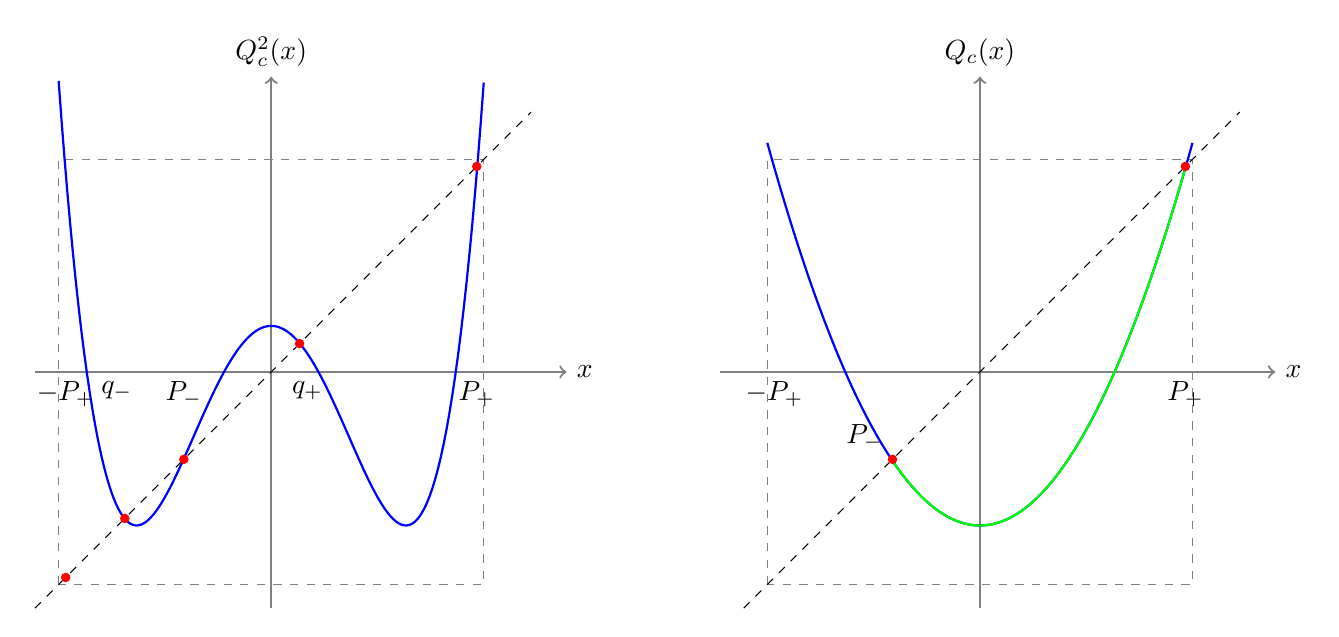
\begin{tikzpicture}[scale=1.5]
			% Lado Izquierdo: Q_c^2(x)
			\begin{scope}[shift={(0,0)}]
				\draw[->, thick, gray] (-2,0) -- (2.5,0) node[right, black] {$x$};
				\draw[->, thick, gray] (0,-2) -- (0,2.5) node[above, black] {$Q_c^2(x)$};
				
				% Cuadro delimitador referencial
				\draw[dashed, gray] (-1.8,-1.8) rectangle (1.8,1.8);
				\draw[dashed, black] (-2,-2) -- (2.2,2.2); % Diagonal y=x
				
				% Función W simulada para c = -1.3 (aproximado visual)
				\draw[thick, blue, domain=-1.8:1.8, samples=150] plot ({\x}, {(\x*\x - 1.3)*(\x*\x - 1.3) - 1.3});
				
				% Marcas en el eje X
				\node[below] at (-1.74, 0) {$-P_+$};
				\node[below, xshift=-0.1cm] at (-1.24, 0) {$q_-$};
				\node[below] at (-0.74, 0) {$P_-$};
				\node[below, xshift=0.1cm] at (0.24, 0) {$q_+$};
				\node[below] at (1.74, 0) {$P_+$};
				
				% Puntos de intersección
				\filldraw[red] (-1.74,-1.74) circle (1pt);
				\filldraw[red] (-1.24,-1.24) circle (1pt);
				\filldraw[red] (-0.74,-0.74) circle (1pt);
				\filldraw[red] (0.24,0.24) circle (1pt);
				\filldraw[red] (1.74,1.74) circle (1pt);
			\end{scope}
			
			% Lado Derecho: Q_c(x)
			\begin{scope}[shift={(6,0)}]
				\draw[->, thick, gray] (-2.2,0) -- (2.5,0) node[right, black] {$x$};
				\draw[->, thick, gray] (0,-2) -- (0,2.5) node[above, black] {$Q_c(x)$};
				
				% Cuadro delimitador referencial
				\draw[dashed, gray] (-1.8,-1.8) rectangle (1.8,1.8);
				\draw[dashed, black] (-2,-2) -- (2.2,2.2); % Diagonal y=x
				
				% Parábola Q_c(x)
				\draw[thick, blue, domain=-1.8:1.8, samples=100] plot ({\x}, {\x*\x - 1.3});
				
				% Resaltado en verde (la parte que cae debajo de y=x)
				\draw[thick, green, domain=-0.74:1.74, samples=100] plot ({\x}, {\x*\x - 1.3});
				
				% Marcas en el eje X
				\node[below] at (1.74, 0) {$P_+$};
				\node[below] at (-1.74, 0) {$-P_+$};
				
				% Puntos de intersección
				\filldraw[red] (-0.74,-0.74) circle (1pt) node[above left, black] {$P_-$};
				\filldraw[red] (1.74,1.74) circle (1pt);
			\end{scope}
		\end{tikzpicture}
	}
	\caption{Dinámica gráfica para $Q_c$ cuando $c \in (-5/4, -3/4)$. La gráfica de $Q_c^2(x)$ corta 4 veces la diagonal $y=x$, revelando el nacimiento de los puntos periódicos $q_-$ y $q_+$, mientras que la parábola simple $Q_c(x)$ solo corta la diagonal en los puntos fijos $P_-$ y $P_+$.}
\end{figure}

El crecimiento explosivo del número de puntos periódicos puede apreciarse de manera espectacular para el caso límite $c = -2$. Aquí, el mapa llena por completo el cuadro delimitador $[-2, 2] \times [-2, 2]$ y es posible trazar iteraciones superiores empleando una parametrización trigonométrica $Q_{-2}^n(x) = 2\cos(2^n \arccos(x/2))$.

\begin{figure}[htbp]
	\centering
	\resizebox{\textwidth}{!}{
		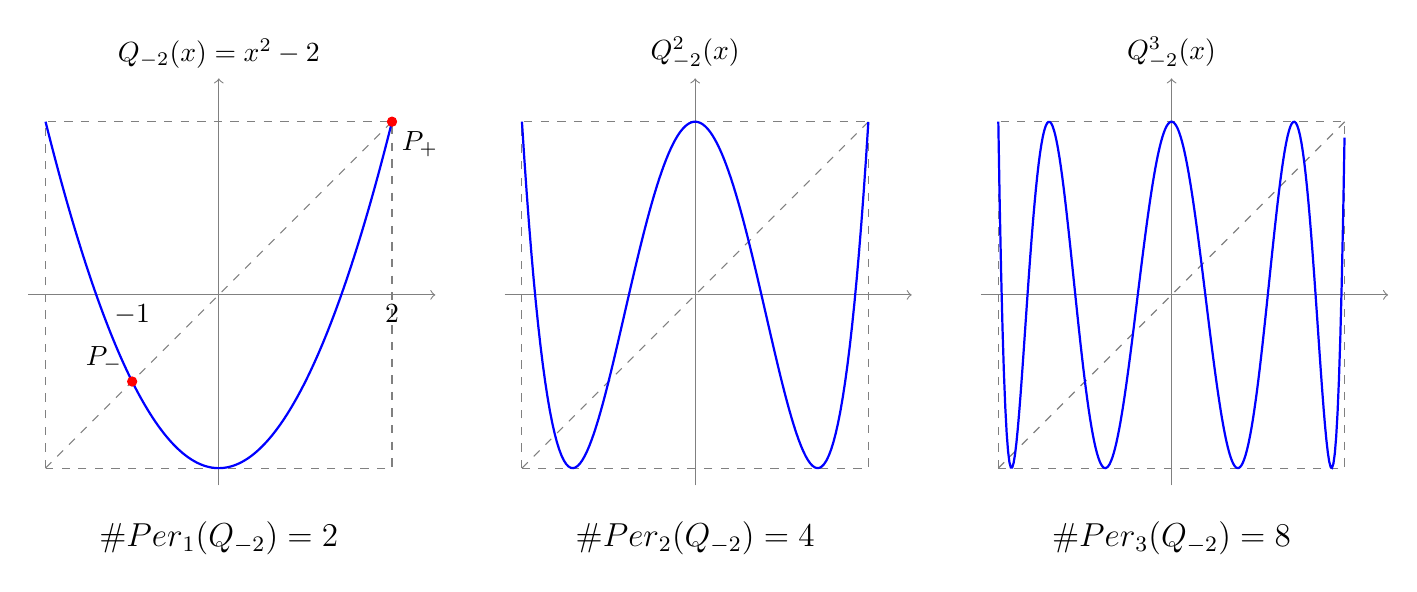
\begin{tikzpicture}[scale=1.1]
			% Iteración n=1
			\begin{scope}[shift={(0,0)}]
				\draw[->, gray] (-2.2,0) -- (2.5,0);
				\draw[->, gray] (0,-2.2) -- (0,2.5) node[above, black] {$Q_{-2}(x) = x^2-2$};
				\draw[dashed, gray] (-2,-2) rectangle (2,2);
				\draw[dashed, gray] (-2,-2) -- (2,2);
				
				\draw[thick, blue, domain=-2:2, samples=150] plot ({\x}, {2*cos(2*acos(\x/2))});
				
				\filldraw[red] (-1,-1) circle (1.5pt) node[above left, black] {$P_-$};
				\filldraw[red] (2,2) circle (1.5pt) node[below right, black] {$P_+$};
				\node[below] at (-1,0) {$-1$};
				\node[below] at (2,0) {$2$};
				
				\node[below, font=\large] at (0, -2.5) {$\# \text{Per}_1(Q_{-2}) = 2$};
			\end{scope}
			
			% Iteración n=2
			\begin{scope}[shift={(5.5,0)}]
				\draw[->, gray] (-2.2,0) -- (2.5,0);
				\draw[->, gray] (0,-2.2) -- (0,2.5) node[above, black] {$Q_{-2}^2(x)$};
				\draw[dashed, gray] (-2,-2) rectangle (2,2);
				\draw[dashed, gray] (-2,-2) -- (2,2);
				
				\draw[thick, blue, domain=-2:2, samples=150] plot ({\x}, {2*cos(4*acos(\x/2))});
				
				\node[below, font=\large] at (0, -2.5) {$\# \text{Per}_2(Q_{-2}) = 4$};
			\end{scope}
			
			% Iteración n=3
			\begin{scope}[shift={(11,0)}]
				\draw[->, gray] (-2.2,0) -- (2.5,0);
				\draw[->, gray] (0,-2.2) -- (0,2.5) node[above, black] {$Q_{-2}^3(x)$};
				\draw[dashed, gray] (-2,-2) rectangle (2,2);
				\draw[dashed, gray] (-2,-2) -- (2,2);
				
				\draw[thick, blue, domain=-2:2, samples=250] plot ({\x}, {2*cos(8*acos(\x/2))});
				
				\node[below, font=\large] at (0, -2.5) {$\# \text{Per}_3(Q_{-2}) = 8$};
			\end{scope}
		\end{tikzpicture}
	}
	\vspace{0.5cm}
	
	\centering\textbf{\Large En general, $\quad \# \text{Per}_n(Q_{-2}) = 2^n$}
	\caption{Intersecciones de $Q_{-2}^n(x)$ con la recta identidad. Cada incremento en $n$ duplica las oscilaciones de la función "U", duplicando así las intersecciones y el número de puntos periódicos.}
\end{figure}

Estas propiedades topológicas no son exclusivas de la familia cuadrática; el sistema dinámico que rige $Q_{-2}(x)$ está profundamente interconectado con el mapa logístico y el Shift de Bernoulli a través de relaciones de conjugación topológica.

\begin{figure}[htbp]
	\centering
	\resizebox{0.9\textwidth}{!}{
		\begin{tikzpicture}[
			node distance=2.5cm and 3.5cm,
			box/.style={draw, thick, rounded corners, align=center, minimum width=4cm, minimum height=1.5cm, fill=blue!5},
			arrow/.style={<->, thick, >=Stealth, shorten >=2pt, shorten <=2pt},
			arrow_down/.style={->, thick, >=Stealth, shorten >=2pt, shorten <=2pt}
			]
			
			% Nodos
			\node[box] (Q) { $Q_{-2}: [-2, 2] \to [-2, 2]$ \\ $x \mapsto x^2 - 2$ };
			\node[box, below=of Q] (f) { $f: [0, 1] \to [0, 1]$ \\ $x \mapsto 4x(1-x)$ };
			\node[box, right=of Q, yshift=-1.5cm] (g) { $g: [0, 1] \to [0, 1]$ \\ 
				$x \mapsto \begin{cases} 2x, & x \le 1/2 \\ 2-2x, & x > 1/2 \end{cases}$ };
			
			\node[box, below=of g, fill=red!5] (sigma) { $\sigma: \Sigma_2^+ \to \Sigma_2^+$ \\ \text{Shift de Bernoulli} };
			
			% Conexiones con align=center
			\draw[arrow] (Q) -- (f) node[midway, left, font=\bfseries, align=right] {Topológicamente\\Conjugado};
			\draw[arrow] (f) to[out=0, in=270] node[midway, below right, font=\bfseries, align=left] {Topológicamente\\Conjugado} (g);
			\draw[arrow_down] (sigma) -- (g) node[midway, right, font=\bfseries, align=left] {Es un factor de\\(Semi-conjugado)};
			
			% Flecha extra indicando relación de Q a g
			\draw[arrow] (Q) to[out=0, in=90] node[midway, above right, font=\bfseries, align=left] {Topológicamente\\Conjugado} (g);
			
		\end{tikzpicture}
	}
	\caption{Diagrama de conjugación entre mapas caóticos clásicos. Todos estos mapas comparten la misma entropía topológica y el crecimiento de $2^n$ puntos periódicos, siendo el Shift de Bernoulli la representación simbólica fundamental del caos determinista subyacente.}
\end{figure}

% =========================================================================
% --- FIN INPUT SEMANA 6 ---
% =========================================================================